\documentclass[__main__.tex]{subfiles}

\begin{document}

\section{Множество степеней свободы триангуляции $T_h$. Оператор табуляции для триангуляции $T_h$. Базисная функция конечно-элементного пространства $X_h$ для стандартных конечных элементов. Лемма о представлении оператора $X_h$ -интерполяции с помощью базисной функции. Теоремы о вложении конечно-элементного пространства $X_h$ в пространство Соболева.}

\begin{definition}
	Пусть $T_h$ - триангуляция на основе стандартных конечных элементов  и пусть введена нумерация(единая - без дублирования) всех степеней свободы из $\Sigma_k \;\; \forall k \in T_h$
\begin{figure}
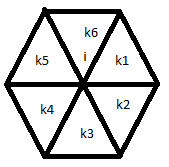
\includegraphics[width=0.4\linewidth]{14.1.png}
\end{figure}\\
$i$-ый узел дл\ каждого треугольника не ненуммеруется каждый раз. \\
Тогда $\Sigma_h = {F_i, i=1..M_h}$ - множество степеней свободны триангуляции $T_h$\\
Пусть $\mathcal{D}_n \in T_h$ - мн-во КЭ-ов, содержащих степень свободы с глобальным номером $n$\\
$\mathcal{D}_i = {K_j, j=1..6}$
\end{definition}

\begin{definition}
	Пусть $\Phi_i = \bigcup_{k \in \mathcal{D_i}}k$, тогда $h_i$ - базисная функция $X_h$, соответствующая глобальному номеру степени свободы $i$:
	\begin{gather*}
		h_i(\tau) =
		\begin{cases}
		\varphi_j^k(\tau)\in \Sigma_k, \; \tau \in \Phi_i \cap K, \; j, \phi_j(a_i)=1\\
		0, \tau \notin \Phi_i
		\end{cases}
	\end{gather*}
\end{definition}

\begin{definition}
	Пусть $\Sigma_h = {F_i, \; i=1..M_n}$, тогда \\
	$T_h(x) = (F_1(x) ... F_{M_n}(k))^T$ -оператор табуляции в $X_h$
\end{definition}

\begin{theorem}
	Пусть $T_h$ - триангуляция на основе стандартных КЭ $(K, P_k, \Sigma_k)$\\
	Пусть $\Sigma_k$-множество степеней свободы всей триангуляции 
	$$
	\Sigma_k = {F_i, \; i-1..M_n}
	$$
	Тогда $\Pi_h \circ x = \sum_{i=1}^{M_n}F_i(x)h_i(\tau), \;\; \forall x: x|_k \in C^{S_k}(k)$,\\
	где $h_i$-базисна функция степени свободы с глобальным номером $i$
\end{theorem}
\begin{proof}
	Пусть $\mathcal{D}OF(k)$-множество глобальных номеров степеней свободы для КЭ $K \in T_h$\\
	Тогда 
	$$
	(\Pi_n \circ x)|_k = \sum_{i \in \mathcal{D}OF(k)}F_i(x)h_i = \sum_{i=1}^{N_k}f_i(x)\varphi_i = \Pi_k \circ x
		$$
\end{proof}

\begin{theorem}[О вложении $X_h$ в $H^1(\Omega)$]
	Пусть $T_h$-триангуляция липшицевой области $\Omega$
	\begin{gather*}
		u(k, P_k, \Sigma_k) - KЭ\\
		P_k\subset H^1(K) \text{и} X_n \subset C(\overline{\Omega}) \\
		\text{Тогда} X_n \subset H^1(\Omega)
	\end{gather*}
\end{theorem}
\begin{proof}
	\begin{center}
	Так как $P_k \subset H^1(\Omega),$ то $\forall p \in P_k$\\
	$\int_k \partial^i p\mu d\tau = -\int_k p\partial^i \mu d\tau + \int_\partial{k} p\mu n_i d\tau$\\
	$n_i$ - компонента внешней нормали $\vec{n}$ к $\partial{k}$\\
	$\forall \mu \in C_0^\infty (\Omega)$\\
	Суммируя по $K \in T_h$, получим:
	
	$\int_{\Omega} \partial^{i}p\mu d\tau = -\int_{\Omega}\partial^i \mu d\tau + \sum_{K \in T_h} \int_{\partial{K}}p\mu n_i d\tau$\\
	$\sum_{K \in T_h}\int_{\partial{K}}p\mu n_i d\tau = 0$\\
	$p \in H^1(\Omega) \text{т.е.} X_n \subset H^1(\Omega)$
	\end{center}
\end{proof}
\end{document}
